\addchapheadtotoc
\chapter{Applied Radiation Model}\label{chapter:Example}
The complexity of the radiation solver resulting from both its theoretical foundation as well as its computational implementation calls for an extensive series of validation and performance studies.

Three test geometries are presented in this chapter for verification and profiling using the two methods discussed in section \ref{section:ModelForThisStudy}. The new MCRT models using the bounding volume hierarchy approach will be refered to as MCRT-ArborX, and the model without will be referred to as MCRT-Kokkos. 
A well-established Fortran implementation developed over the course of many years will be used for comparison, and will be refered to as MCRT-Fort.
The configurations include the canonical one-dimensional plane-parallel medium, a three-dimensional backward-facing step combustor, and a three-dimensional Pratt \& Whitney NEO aeronautical combustor. 
These three test cases provide an excellent basis to verify the solution methods and test their performances. 



\section{One dimensional plane-parallel medium}
The plane-parallel medium provides a useful, one dimensional case to test the MCRT code. The geometry is shown in figure \ref{fig:PlaneParallelGeometry}.

The geometry consists of two parallel plates surrounding a radiatively-participating medium. The system is one-dimensional (implemented into OpenFOAM using either ray-reflections along the off-axis boundaries, or through a long stretch in both the Y and Z directions). The simulation is steady, and the walls are black-bodies (perfect absorbers and emitters).
Using this configuration, the user can artificially select an absorption coefficient, $\kappa{}$, medium temperature, $T$, and wall temperatures $T_w$.

Additionally, the relative simplicity of the configuration allows for reduced-complexity numerical solution described in appendix (IN APPENDIX OR PUT HERE?). 
This "analytical" solution can be used for verification of the solver under variable absorption coefficient, temperatures, and scattering coefficient (not included in this model).

The one-dimensional nature of the system also results in the least-ideal scaling for multi-node simulations. \textit{Provides useful understanding of how the runtime and memory usage scale for each solver under worst-case situations.}

\subsection{Results}
Figure \ref{fig:PP_kappatest} presents a comparison of the MCRT solutions alongside the analytical solutions. The configuration is tested under a variety of absorption coefficients, temperatures, and Monte-Carlo ray counts. The various case conditions are presented in table \ref{table:PPcomp}.

\begin{figure}
  \begin{subfigure}{1\textwidth}
  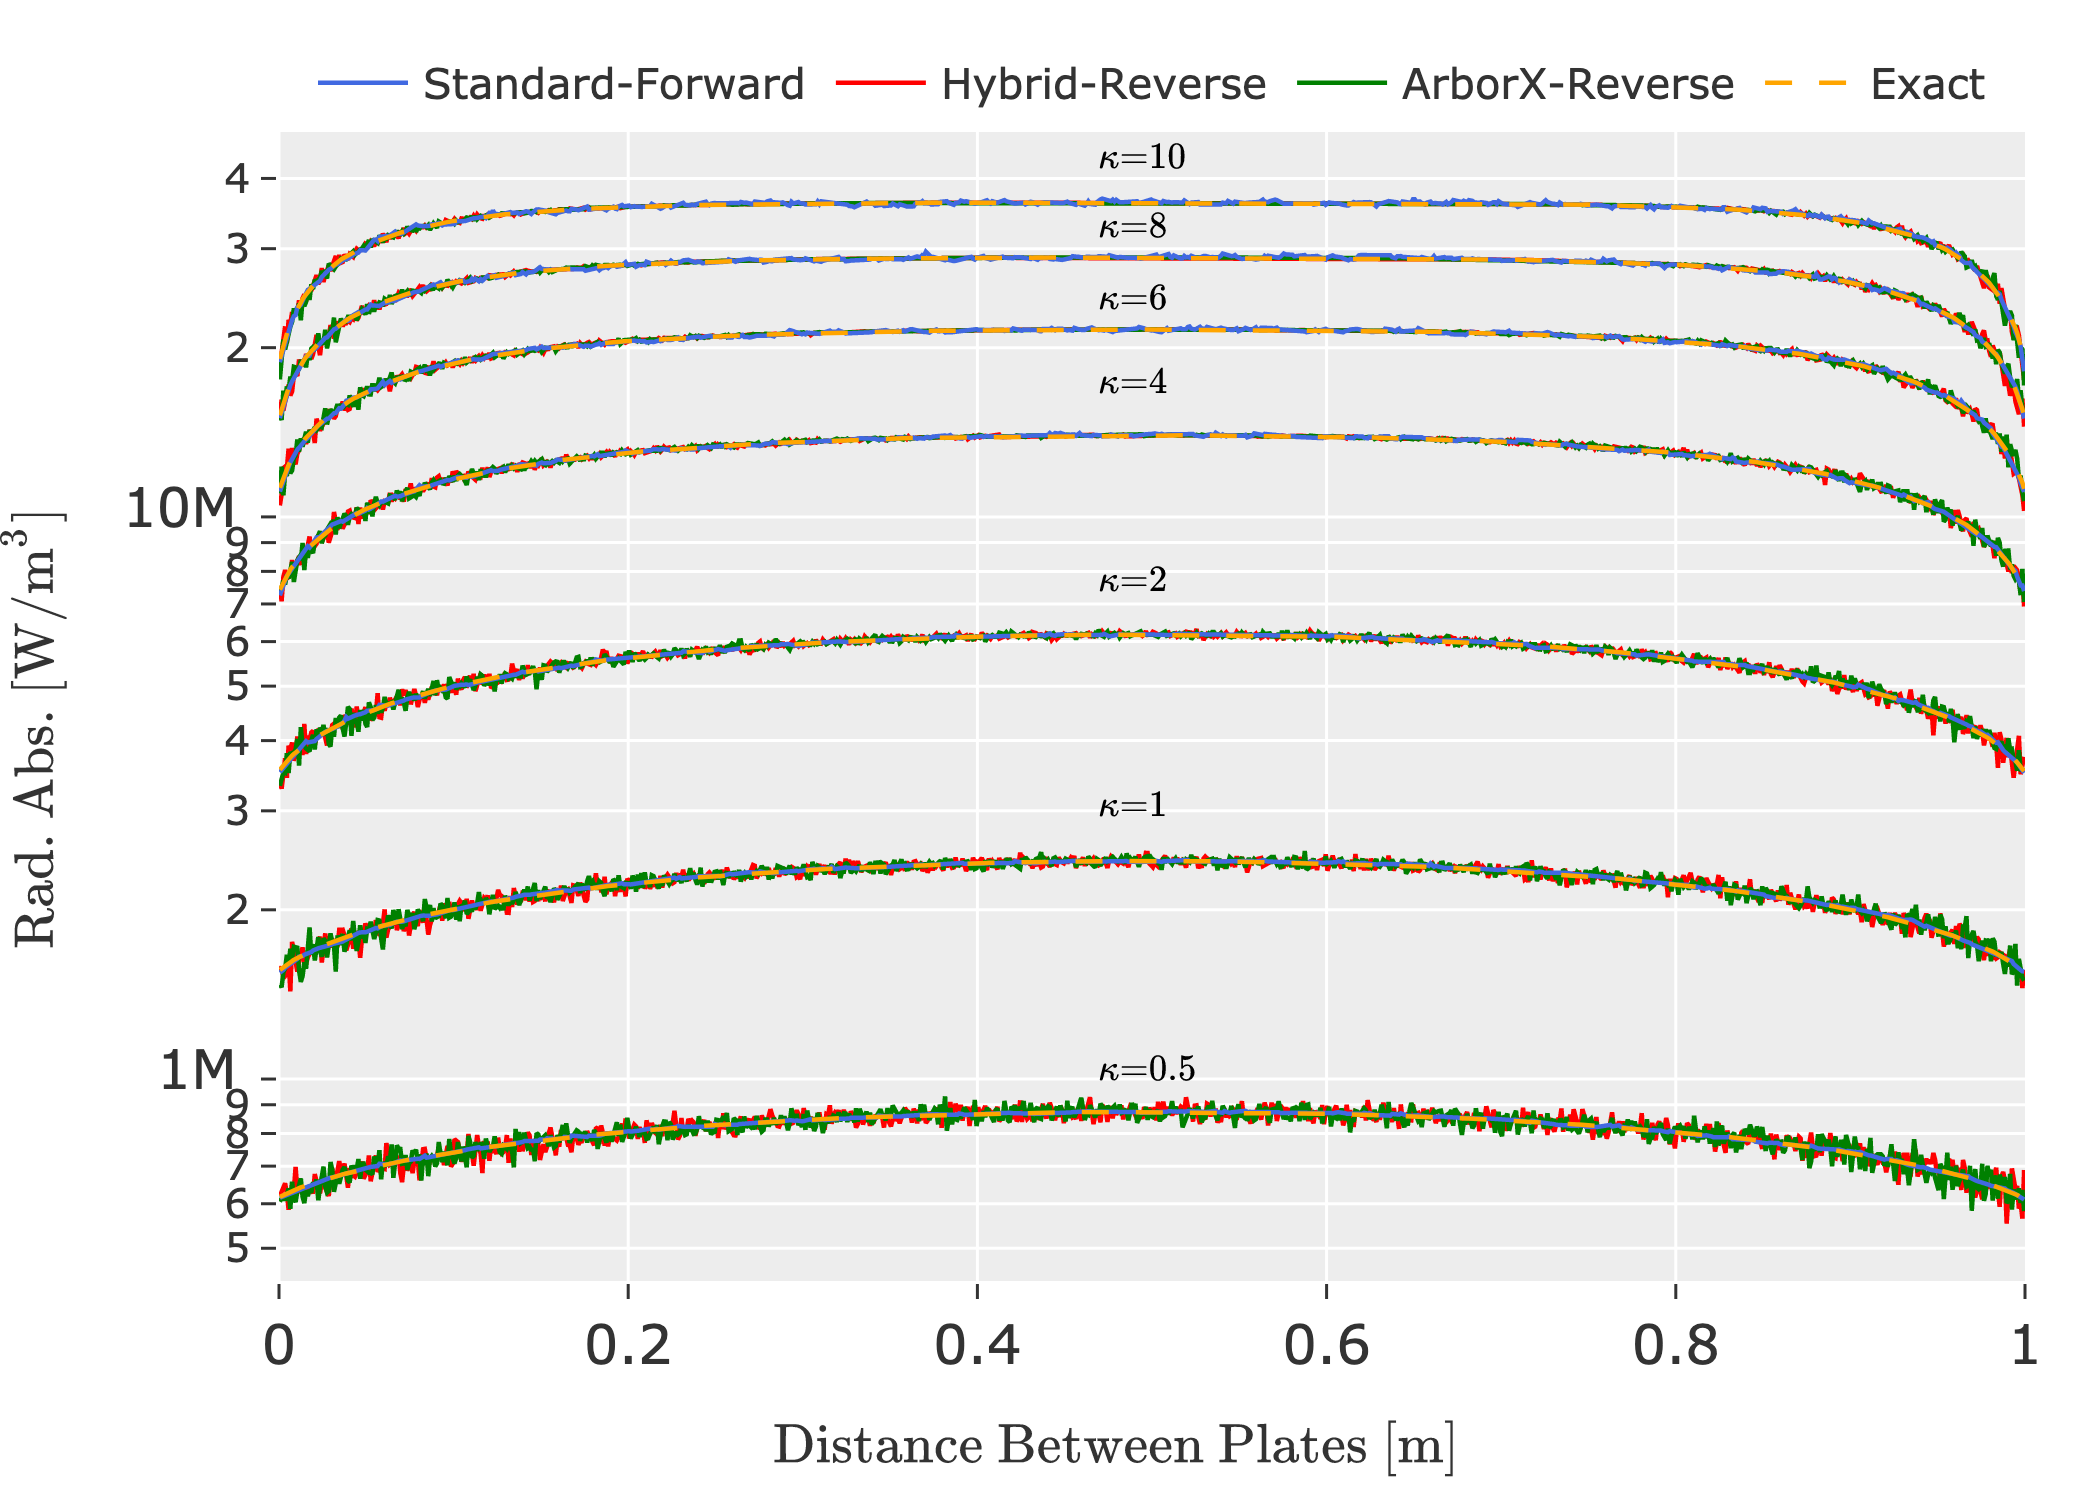
\includegraphics[width=\linewidth]{figures/ch4/PPcomparison1.png}
  \caption{Variable absorption coefficient with T=$2000$K, N$_r$=$1000$, N$_{cells}$=1000.}
  \label{fig:PPcomp_kappa}
  \end{subfigure}
  \begin{subfigure}{1\textwidth}
  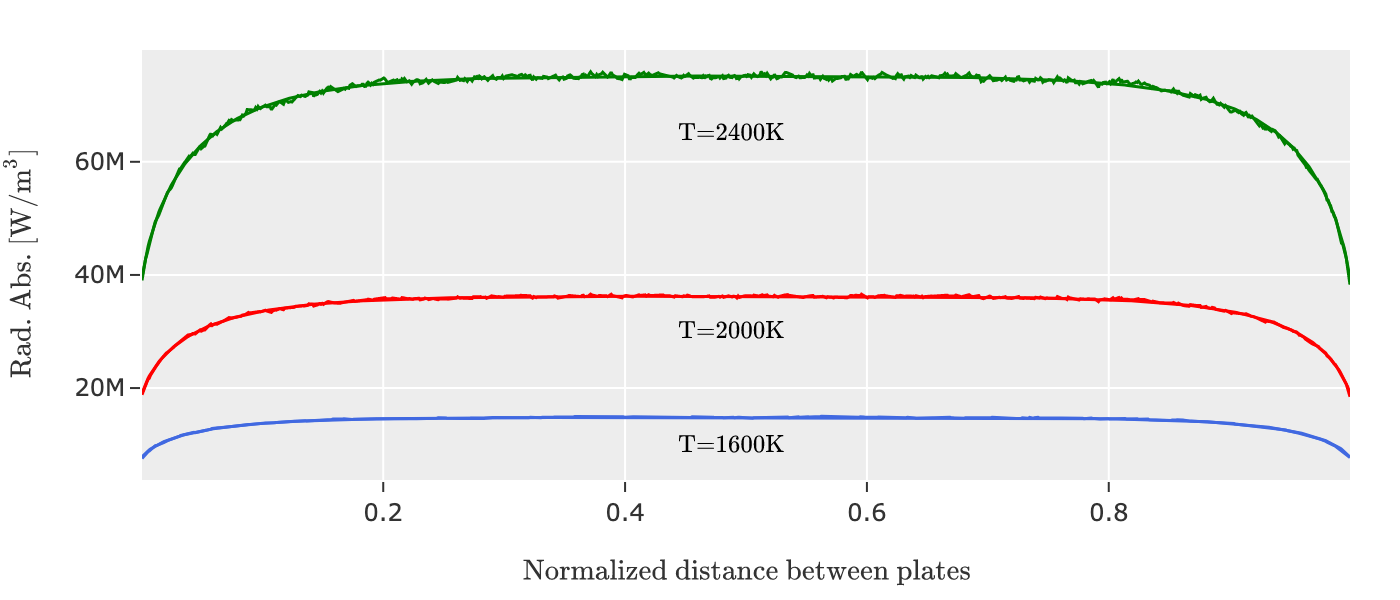
\includegraphics[width=\linewidth]{figures/ch4/PPcomparison2.png}
  \caption{Variable temperature with $\kappa{}$=$10$ m$^{-1}$, N$_r$=$1000$, N$_{cells}$=1000.}
  \label{fig:PPcomp_temp}
  \end{subfigure}
  \begin{subfigure}{1\textwidth}
  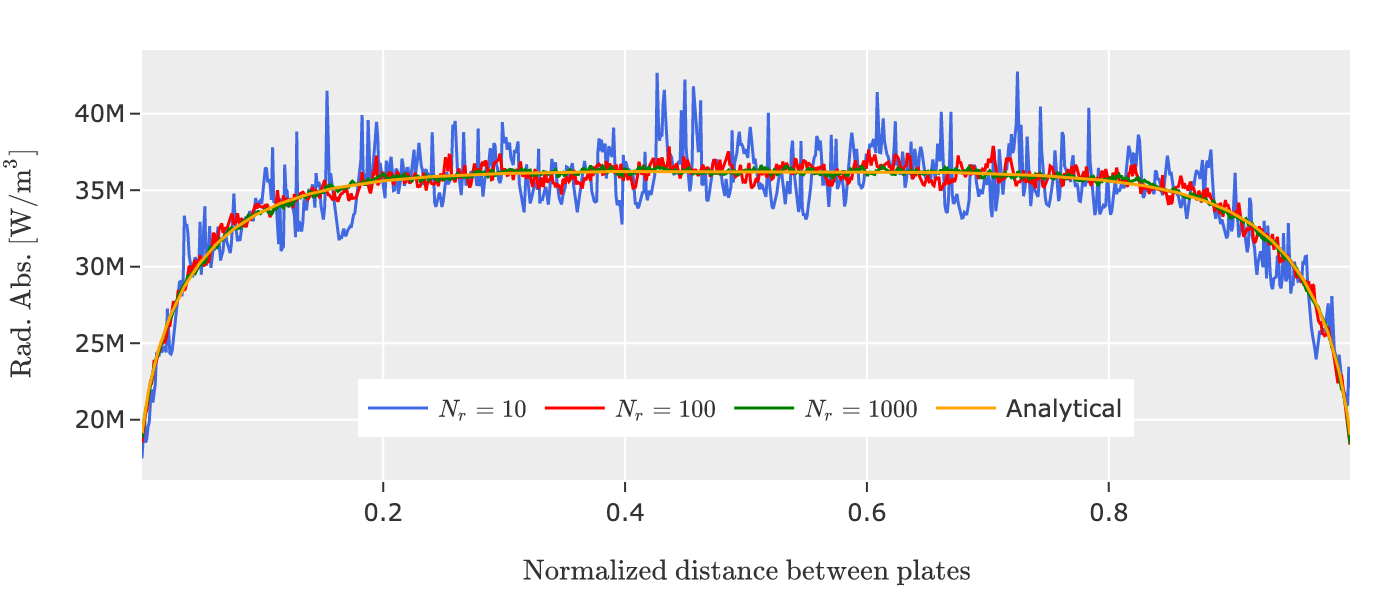
\includegraphics[width=\linewidth]{figures/ch4/PPcomparison3.png}
  \caption{Variable number of rays emitted per cell (N$_r$) with $\kappa{}$=$10$ m$^{-1}$, T=$2000$K, N$_{cells}$=1000.}
  \label{fig:PPcom_nrays}
  \end{subfigure}
  \label{fig:PPcomp}
\end{figure}

Results show excellent comparison between the MCRT and analytical implementations. 
The lower ray counts show a higher degree of variability resulting from the stochastic nature of the MCRT method. 
Increasing absorption coefficient leads in an increase of radiative emission and re-absorption, with re-absorption increasing at a higher rate resulting in a net increase of radiative source.

These expected results demonstrate the requirement for RTE modeling in optically thick media. Not only does radiative emission result in heat loss from computational cells, but also the re-absorption can be high enough to require modeling of the self-absorption process of radiation.

\subsection{Profiling}


\section{Backward-Facing Step Combustor}
The backward-facing step (BFS) combustor is a convenient configuration often used as a simple, repeatable geometry for a variety of studies in fluid dynamics.
Numerous examples exist demonstrating its use for experimental and numerical investigations of turbulent flow~\cite{Armaly1983ExperimentalFlow,Neto1993AStep,Jovic1994Backward-facing5000,Le1997DirectStep}. Combined turbulent and high temperature flow~\cite{Niemann2016Buoyancy-affectedNumber,Xie2017GeometrySteps}, particularly with reactions~\cite{Pouech2021PremixedStep}.
In the relatively few studies that exist, the addition of volumetric heating and composition changes resulting from the exothermic chemical reactions have been shown to influence the thermodynamic state and turbulence intensity of the fluid. Recent interest has emerged regarding the relative influence of radiation and convection along the walls many configurations, and the backward-facing step geometry provides a convenient approach for doing so.

\subsection{Case setup}
\begin{figure}
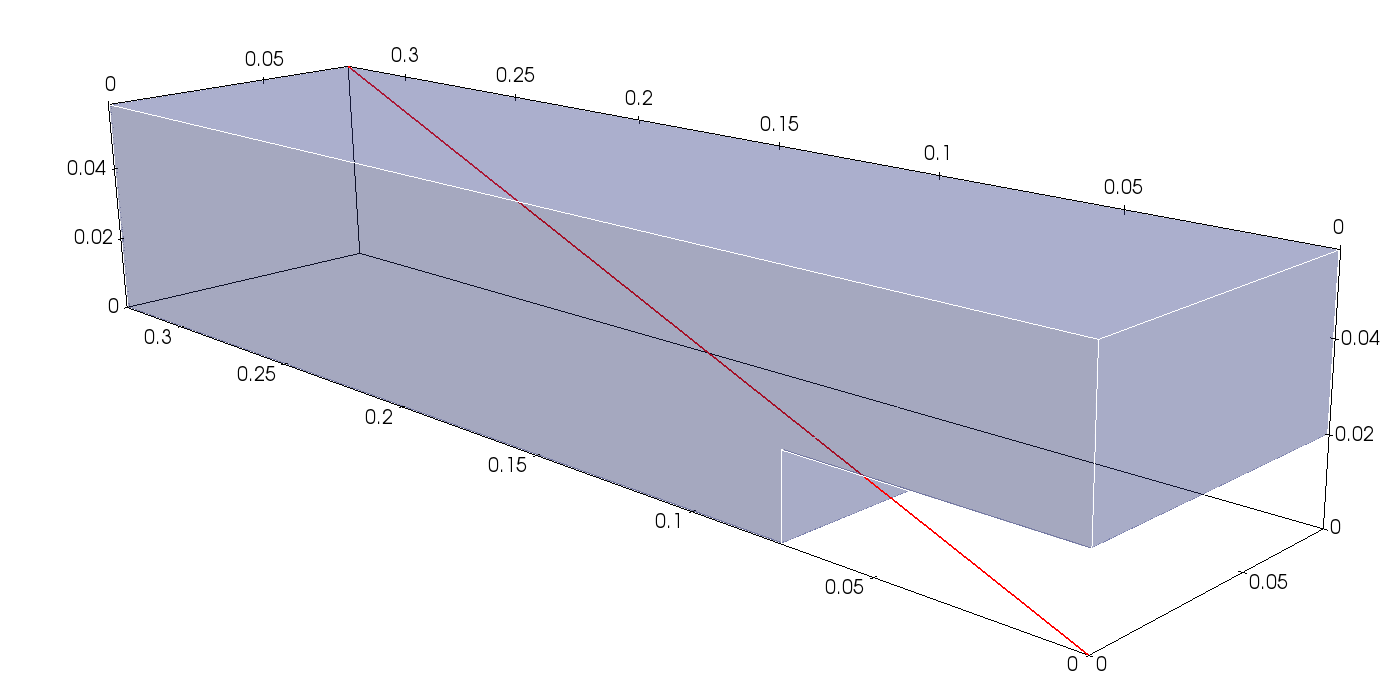
\includegraphics[width=\linewidth]{figures/ch4/BFS_visual.png}
\caption{Dimensions of backward-facing step configuration used in this study in addition to a representative line used to sample radiative properties. All units are in meters. }
\label{fig:BFS_geometry}
\end{figure}

The BFS geometry used in this study is diagrammed in figure \ref{fig:BFS_geometry} based on an experimental configuration at the Pennsylvania State University.
A three-dimensional CFD calculation was performed closely matching the conditions present in the experiment. For this case, no chemically reacting flow is included. 
The flow is present in only vitiated form, where a chemical reaction is initiated in a portion of the flow upstream of the step, and the resulting "dirty" air with high CO$_2$ and H$_2$O content is mixed with unreacted air. 
The mixture reaches the main section at an elevated temperature of up to 850K, appreciably lower than expected temperatures of above 2000K when full reactions are present. 
The simulations account for the elevated temperature, but neglect any further chemical reactions beyond the step, resulting in a purely fluid-mechanical calculation.

Figures \ref{fig:BFS_temperature}, \ref{fig:BFS_streamlines} show temperature and velocity magnitude contours in the BFS. The pressure is atmospheric, and the absorption coefficient is assumed uniform at a value of 0.5 m$^{-1}$ due to the absence of chemical properties in the CFD simulations.

\begin{figure}

\end{figure}
\begin{figure}
  \begin{subfigure}{1\textwidth}
  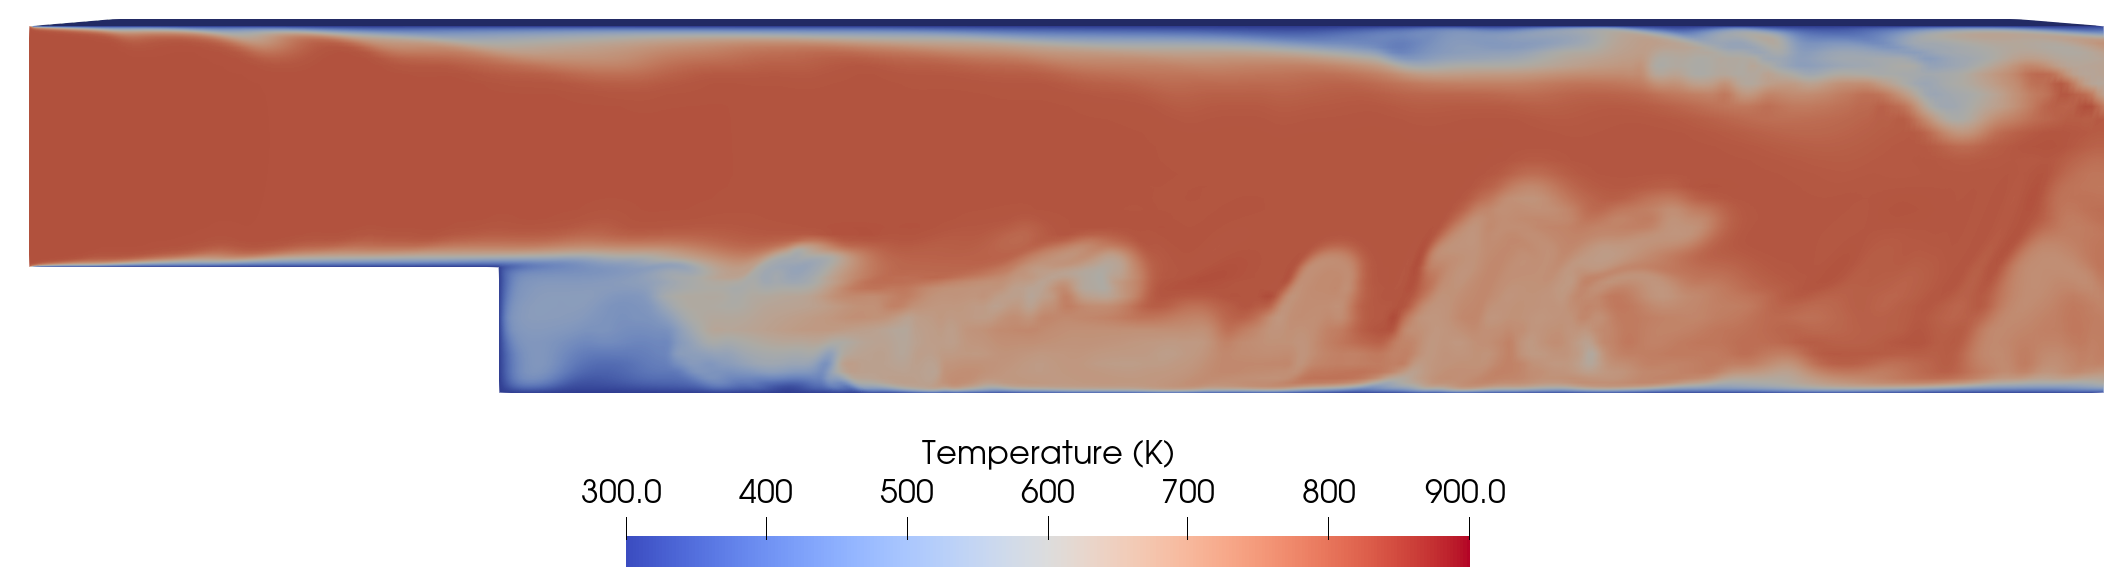
\includegraphics[width=\linewidth]{figures/ch4/BFS_temperature.png}
  \caption{BFS temperature contour along the mid-plane. }
  \label{fig:BFS_temperature}
  \end{subfigure}
  \begin{subfigure}{1\textwidth}
  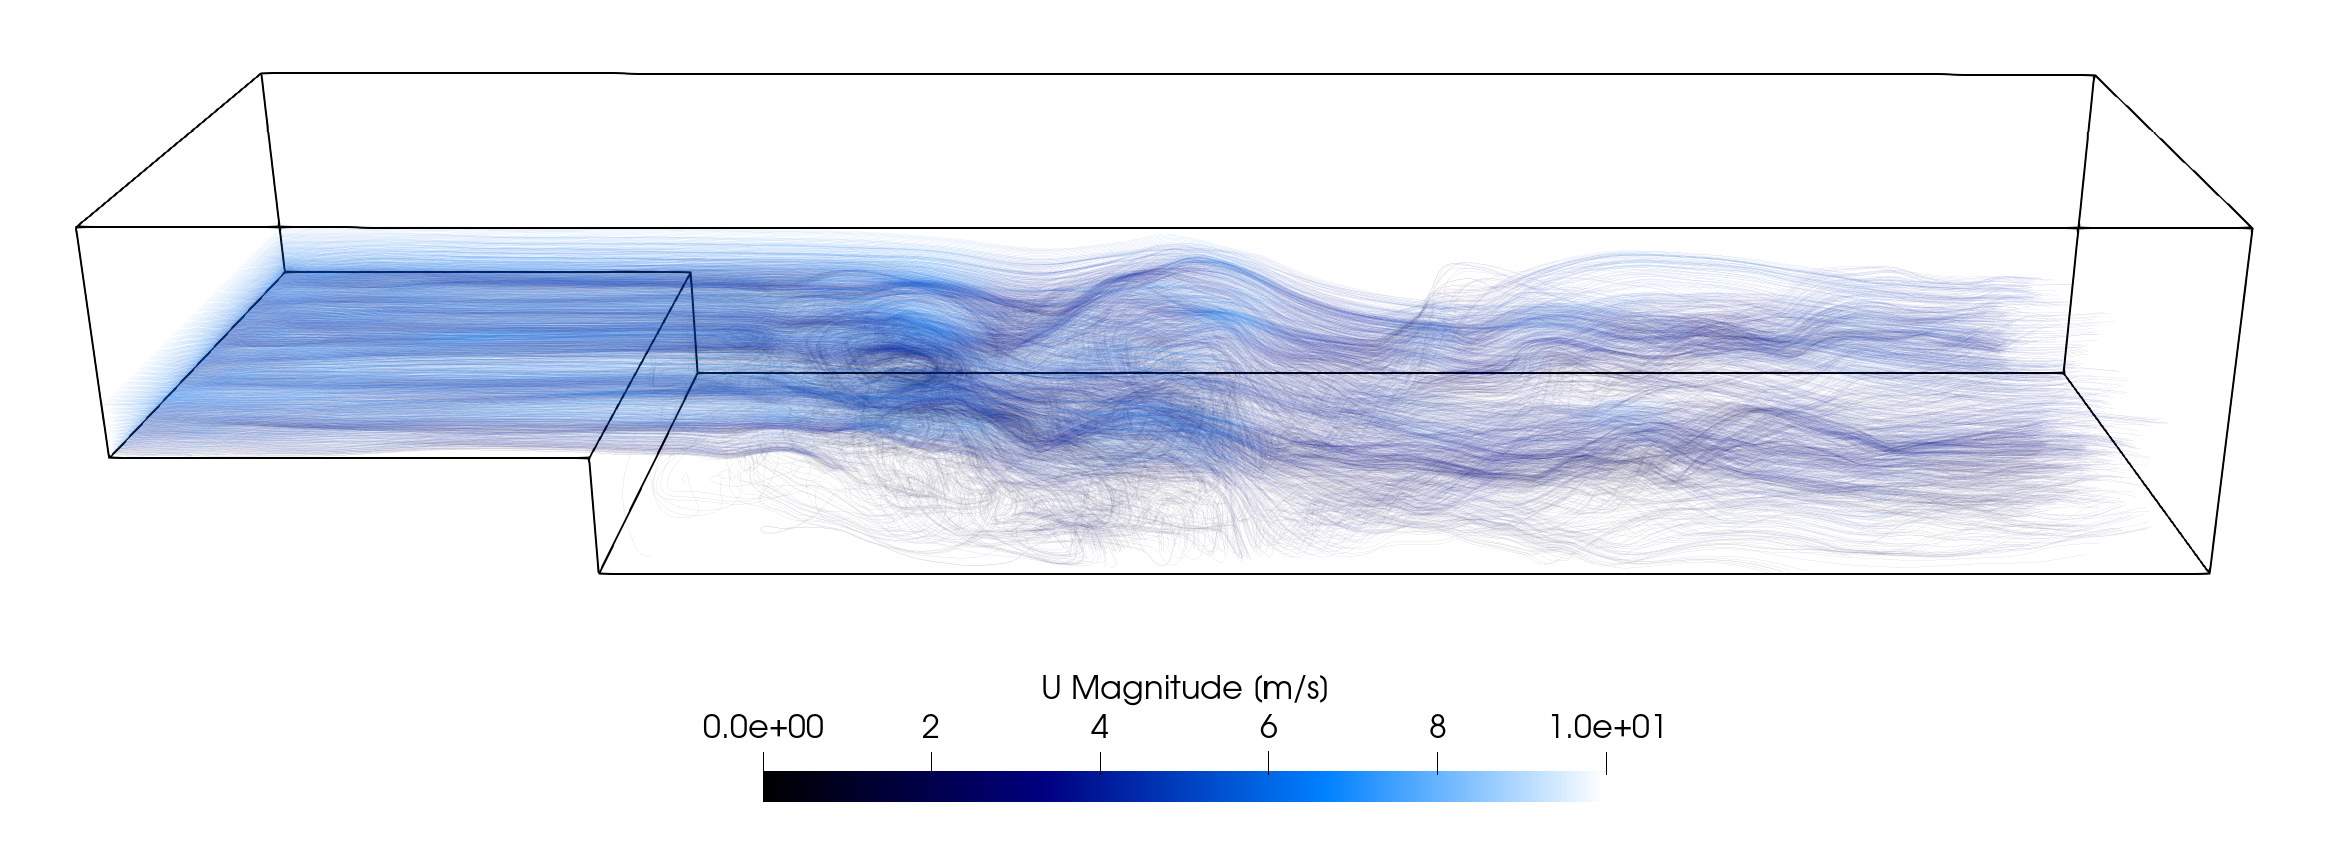
\includegraphics[width=\linewidth]{figures/ch4/BFS_streamlines6.png}
  \caption{Streamlines traced from the entrance of the BFS.}
  \label{fig:BFS_streamlines}
  \end{subfigure}
  \label{fig:BFS_contours}
\end{figure}

\subsection{Results}
A single time-step of the CFD simulation was extracted for a \textit{frozen field analysis} (see chapter \ref{chapter:Introduction}). 
The resulting radiative emission and wall-heat flux iso-contours are shown in figure \ref{fig:BFS_radiationcontours}.


\begin{figure}
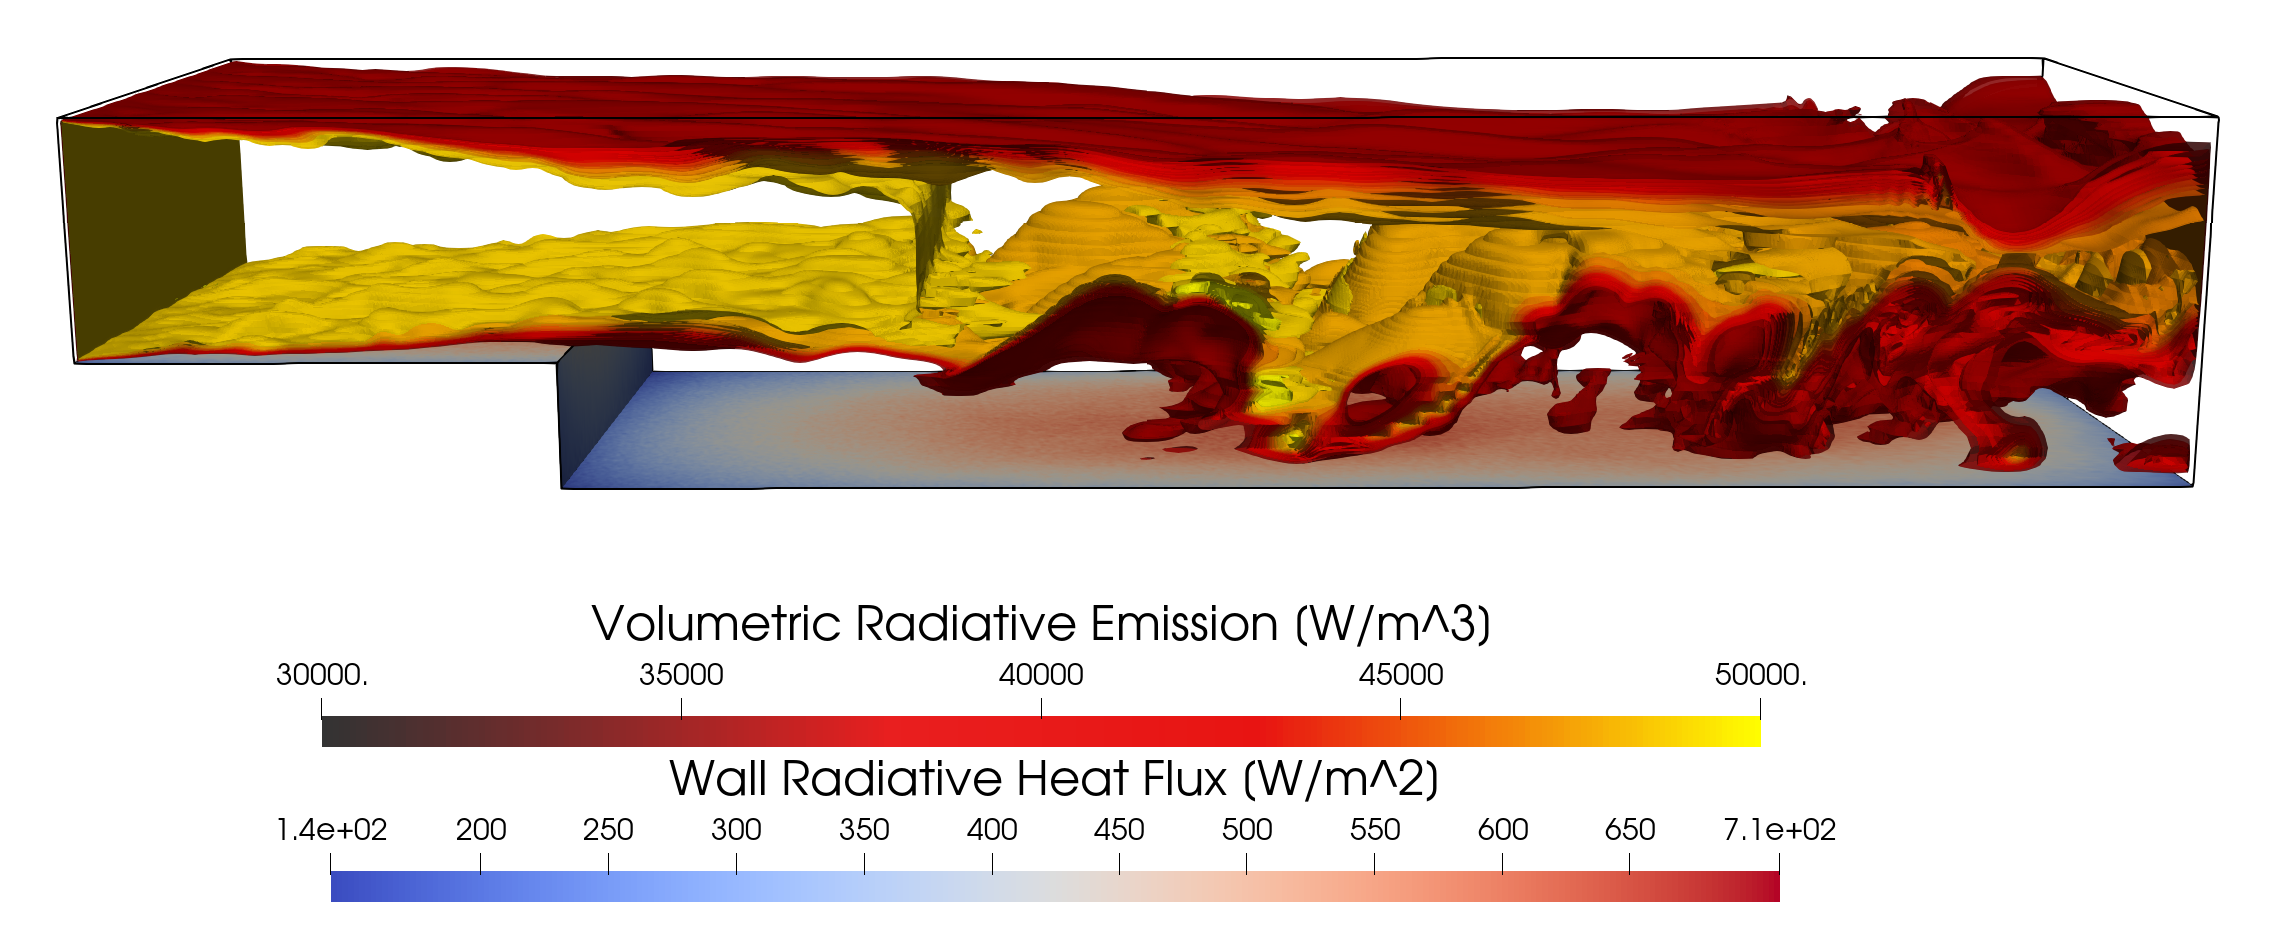
\includegraphics[width=\linewidth]{figures/ch4/BFS_volwallflux3.png}
\caption{Contours of volumetric radiative emission alongside resulting radiative heat flux along the walls.}
\label{fig:BFS_radiationcontours}
\end{figure}

The bulk of radiative emission originates from the re-circulation zone behind the step. Radiation is emitted from the flow and decreases the thermal energy contained in the passing fluid. 
The fluid is then quickly replaced by the new gas at the entrance, which results in a continuous load of radiation incident on the bottom surface of the domain. 

The turbulence present in the recirculation zone is apparent even in the emission contours as a result of the advection of elevated temperatures present. The secondary recirculation zone immediately present adjacent to the step displays lower levels of radiative emission resulting from its slower rate of fresh-gas replenishment.

Figures \ref{fig:BFS_RadAbs}, \ref{fig:RadEmi}, and \ref{fig:RadSrc} show the radiative absorption, emission, and net energy source along the line shown in figure \ref{fig:BFS_geometry} using the different solvers for comparison. 


\begin{figure}
  \begin{subfigure}{1\textwidth}
  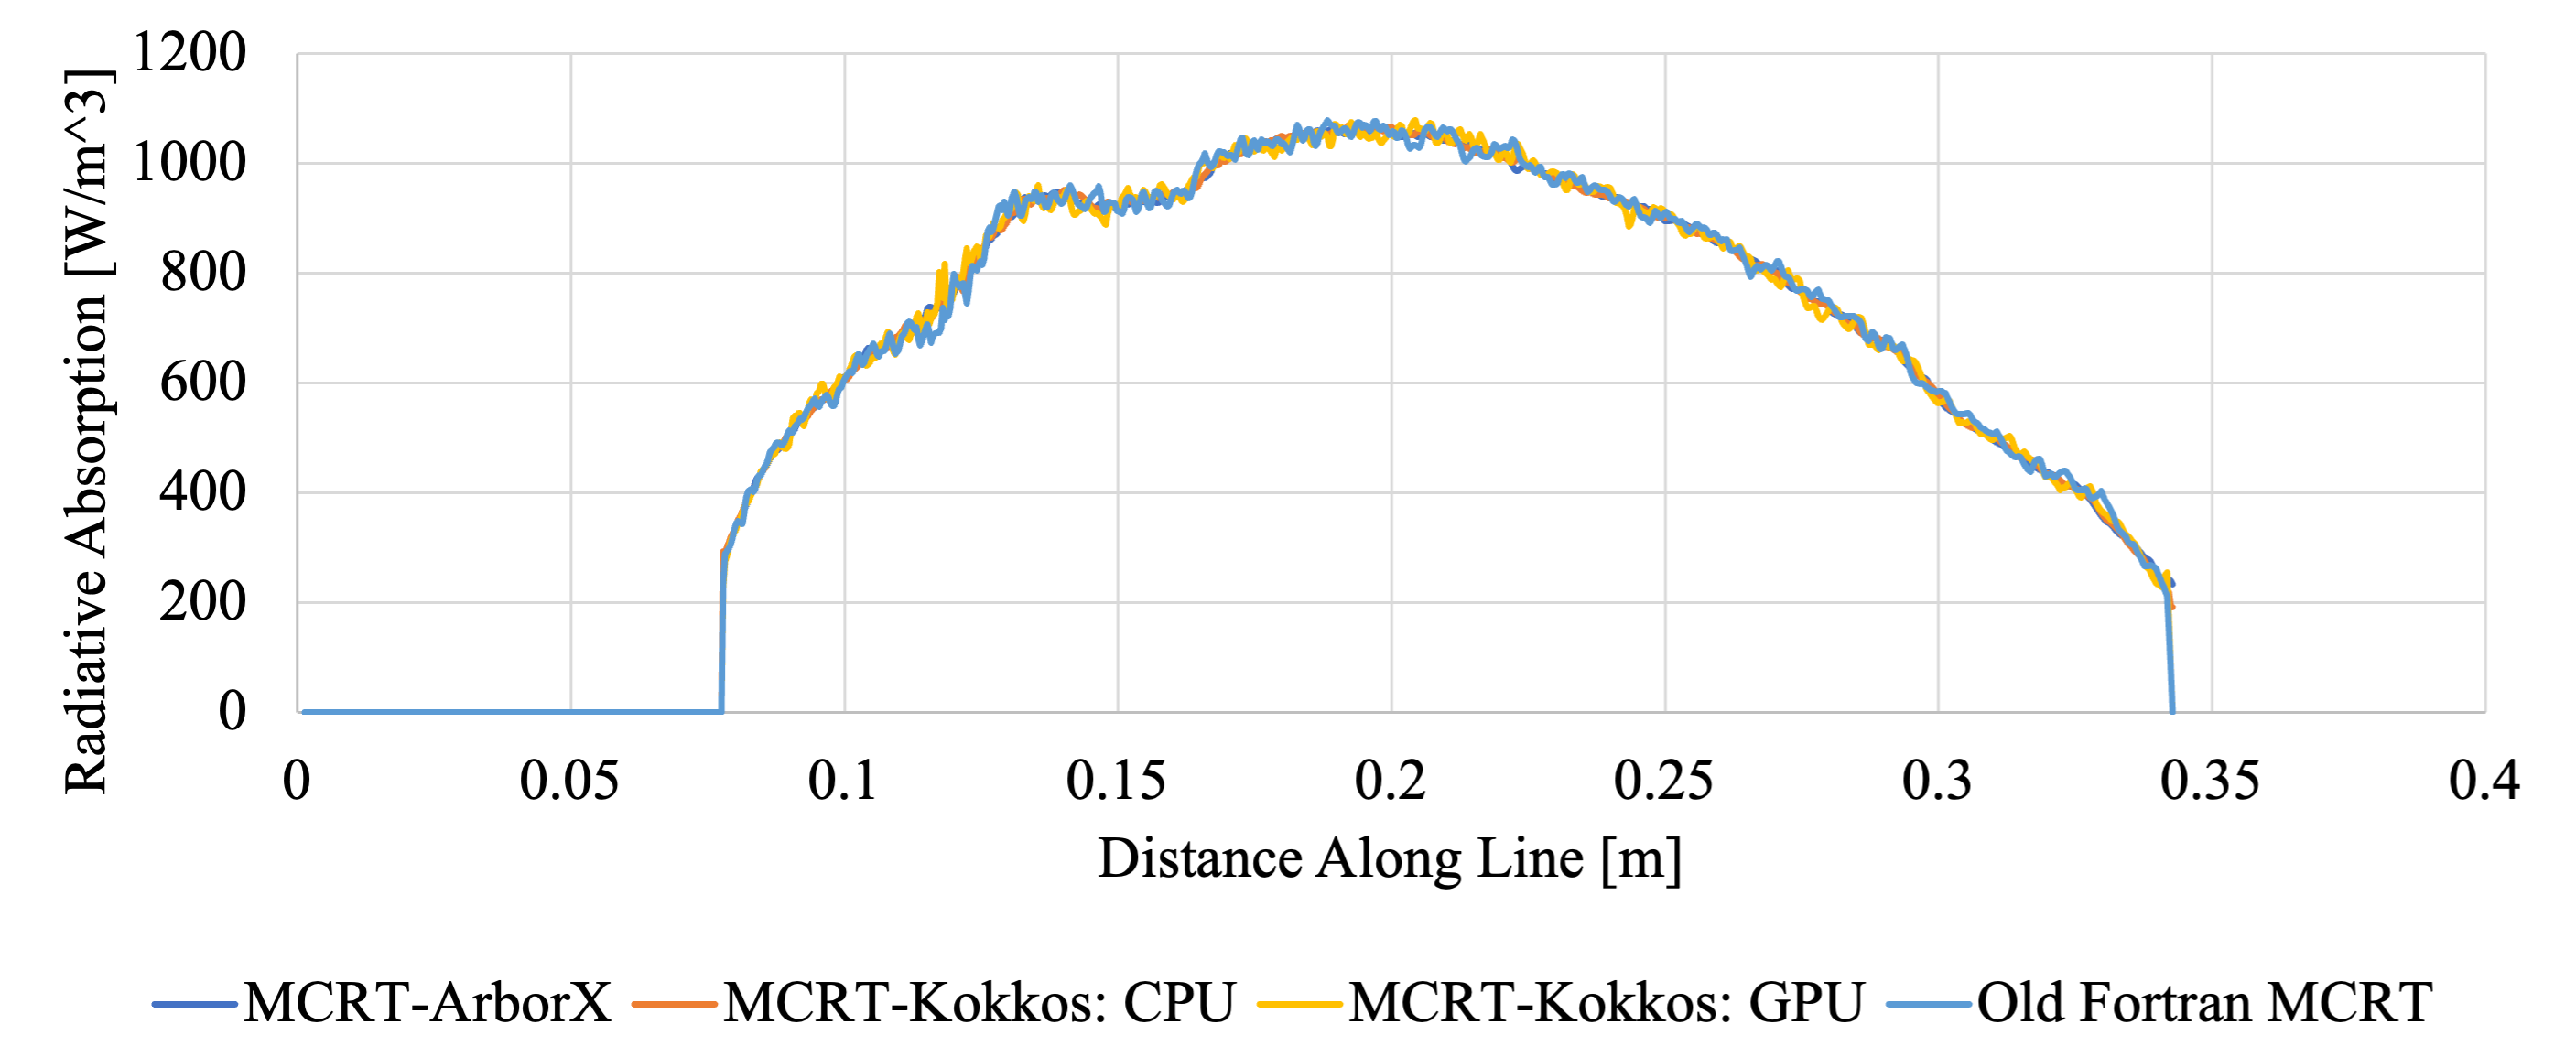
\includegraphics[width=\linewidth]{figures/ch4/LineComparison_RadAbs.png}
  \caption{}
  \label{fig:BFS_RadAbs}
  \end{subfigure}
  \begin{subfigure}{1\textwidth}
  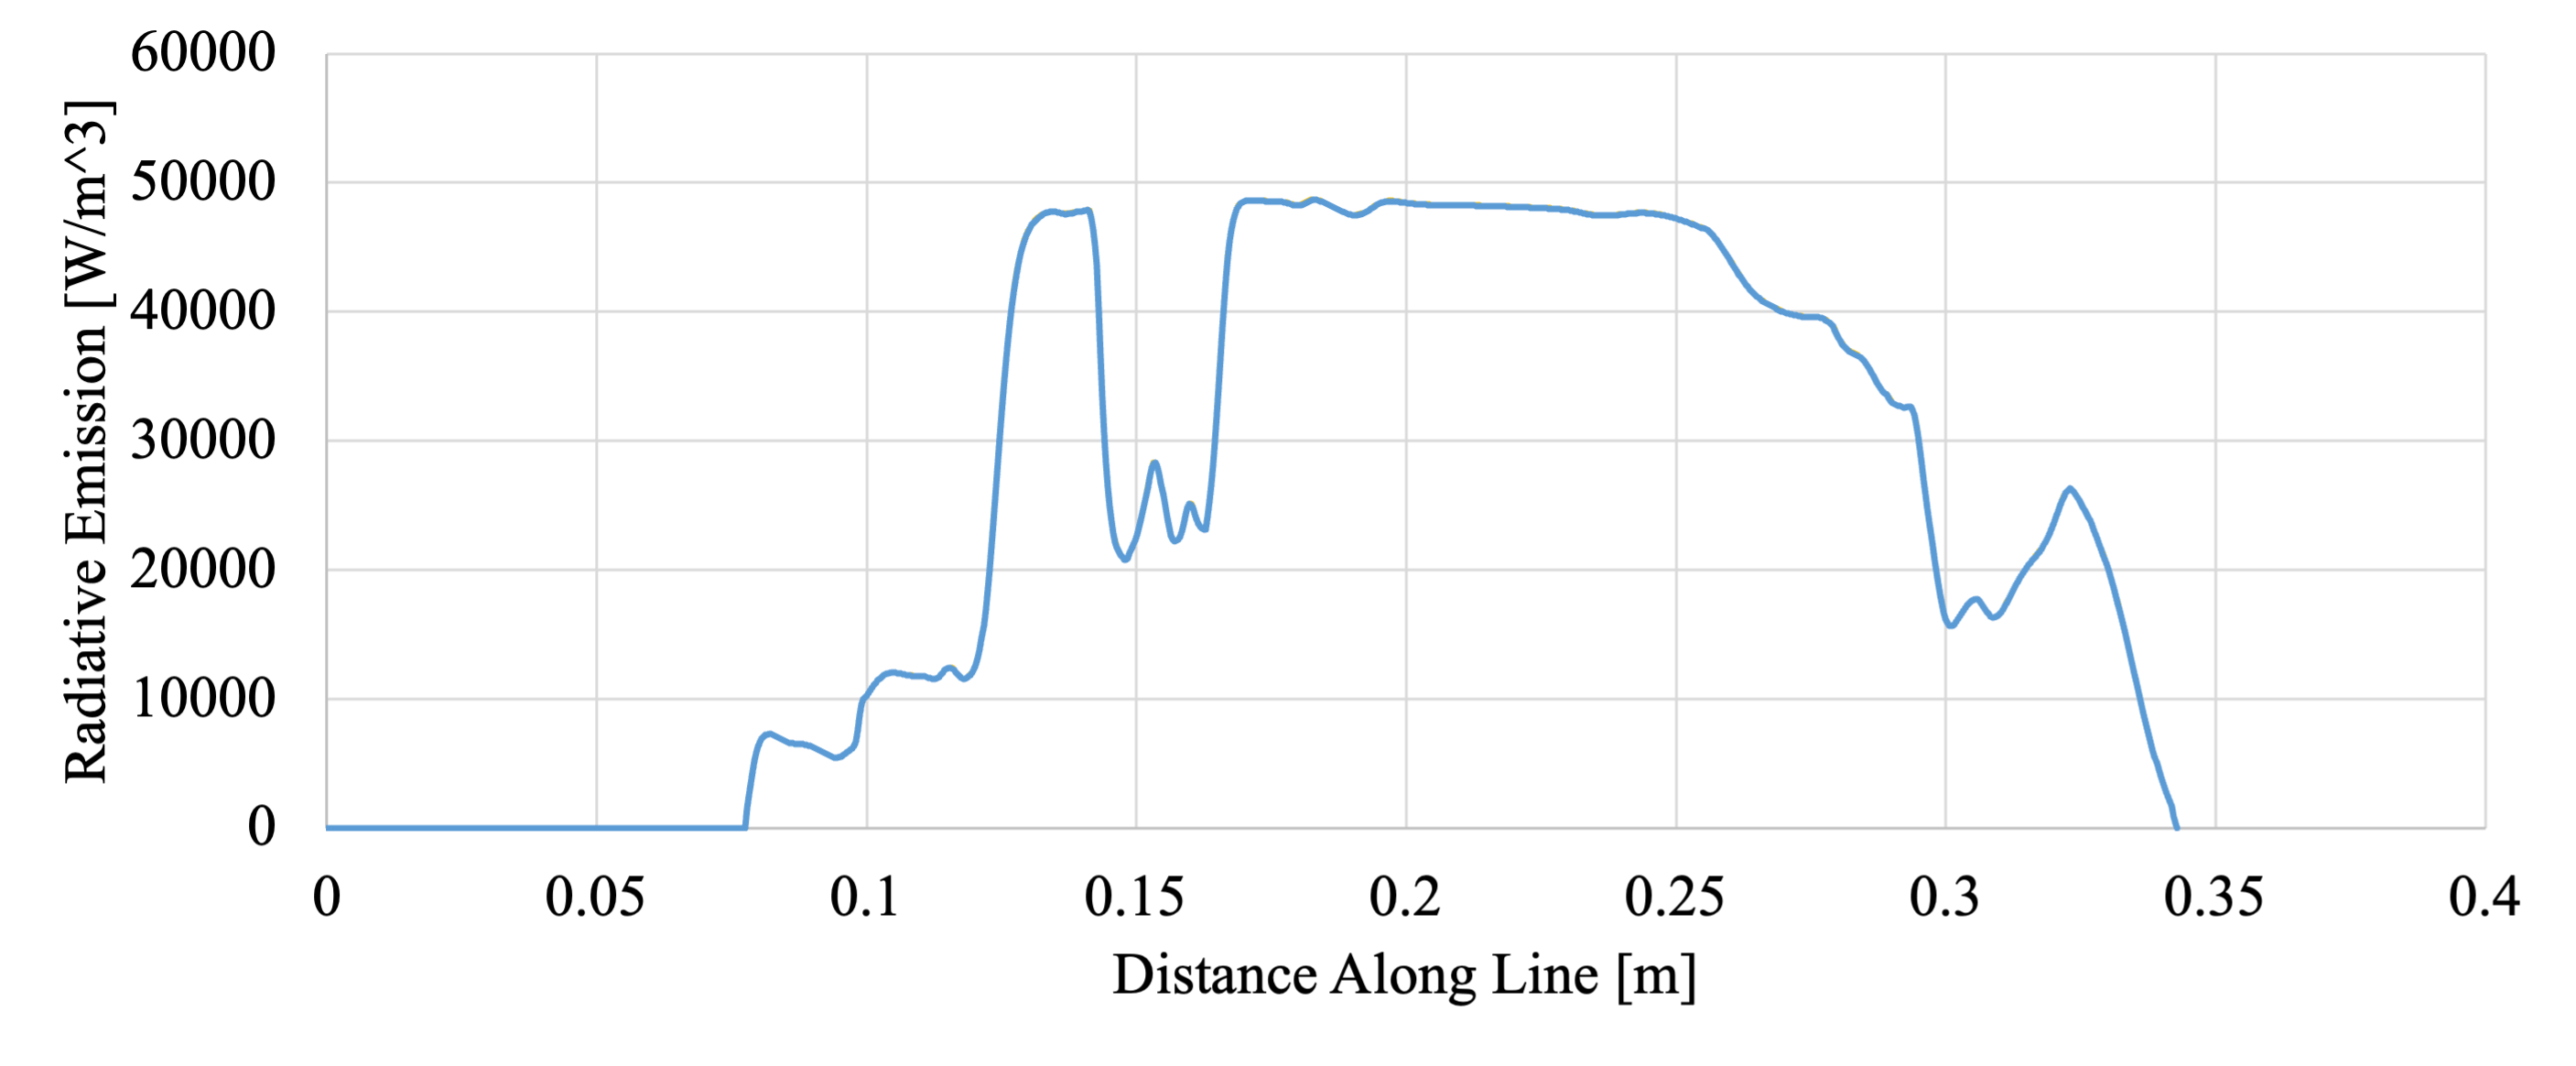
\includegraphics[width=\linewidth]{figures/ch4/LineComparison_RadEmi.png}
  \caption{}
  \label{fig:BFS_RadEmi}
  \end{subfigure}
  \begin{subfigure}{1\textwidth}
  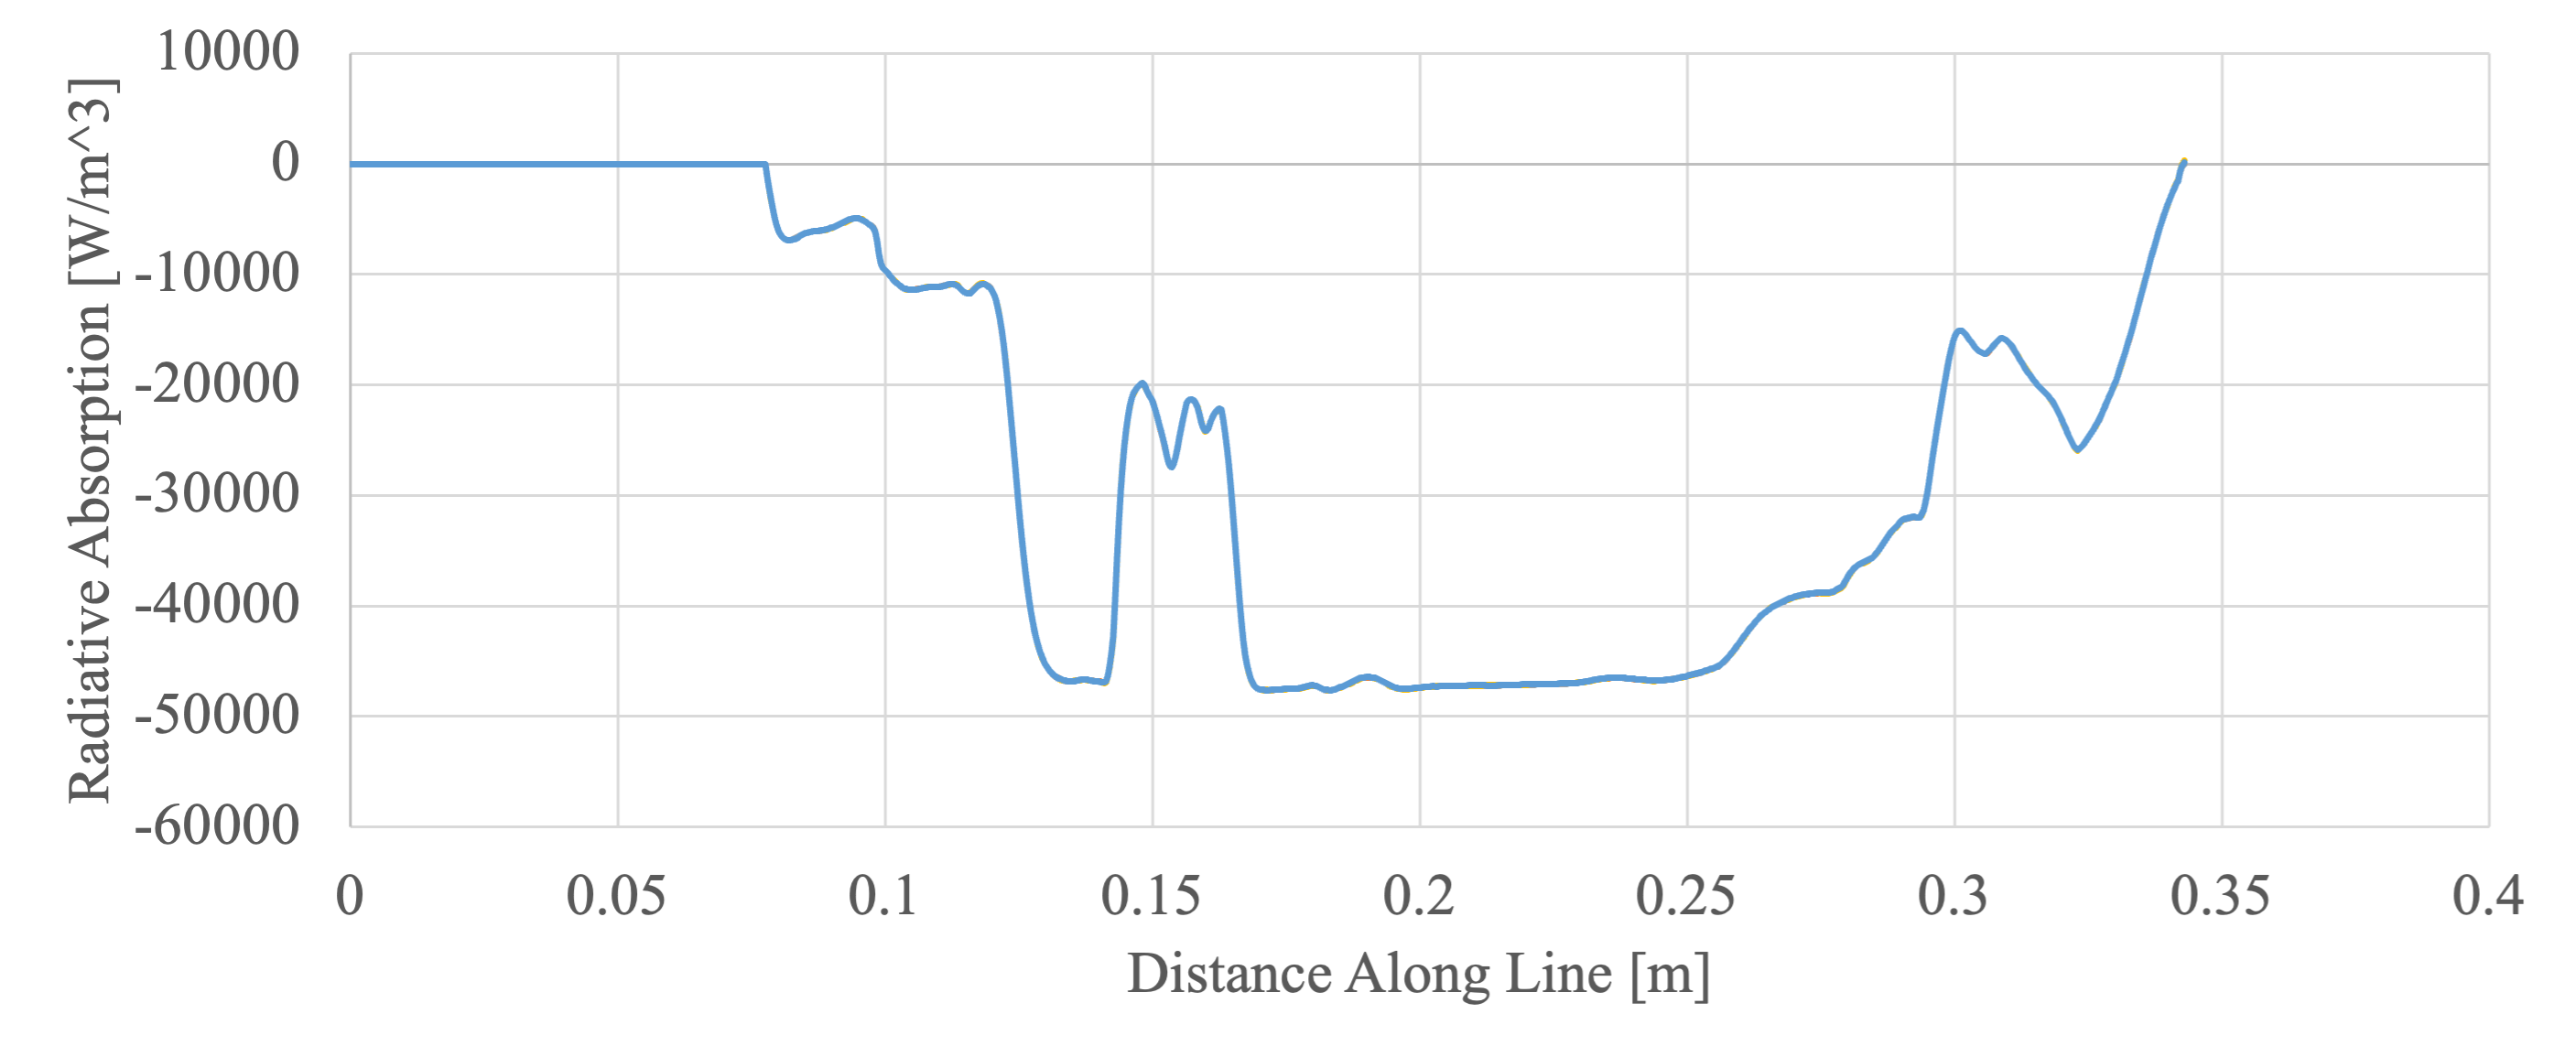
\includegraphics[width=\linewidth]{figures/ch4/LineComparison_RadSrc.png}
  \caption{}
  \label{fig:BFS_RadSrc}
  \end{subfigure}
  \label{fig:PPcomp}
\end{figure}


\subsection{Model Performance}
The radiation was calculated using both new MCRT models as well as a well-established Fortran-based radiation model for comparison. Simulations were performed at the single time-step using both 1 ray per cell and 10 rays per cell for all solvers, and serial, OpenMP and Cuda were tested as Kokkos backends for the new MCRT. 
Simulations were performed using a 72-core Intel(R) Xeon(R) Gold 5220 CPU shared-memory workstation for OpenMP calculations, and Cuda calculations were performed using Nvidia V100 GPUs from the high performance computer Narwhal operated by the defense supercomputing resource center~\cite{something}.

Results are listed in tables \ref{table:BFS_runtime_table_1rpc} and \ref{table:BFS_runtime_table_10rpc} for 1 ray emitted per cell and 10 rays per cell, respectively. The performance of both the MCRT-Kokkos model and the MCRT-ArborX compare extremely well against the MCRT-Fort model for a serial calculation. A runtime improvement of 86\% is already observed before any parallel routines have even been applied.
The dramatic speedup can be attributed to the improved mesh-transfer method implemented in the new MCRT methods. 
Almost no mesh data is duplicated during the mesh transfer process, allowing for minimal delay before the raytracing procedure begins. VERIFY THIS AND COMPARE WITHOUT THE MESH TRANSFER. WHY DOES SERIAL RUN OVER 50X FASTER THAN 30 PROCS?

\begin{table}[h!]
\centering
\begin{tabular}{||c c c c||} 
 \hline
 Parallel Variation & MCRT-Fort & MCRT-Kokkos & MCRT-ArborX \\ [0.5ex] 
 \hline\hline
 Serial & 2687 s & 376 s & - \\ 
 30 CPU Processors & 52.26 s & 22.5 s & - \\
 GPU & N/A & 6.91 s & - \\
 \hline
\end{tabular}
\caption{BFS runtime comparisons with 1 ray emitted per CFD cell. The MCRT-Fort parallel procedure is conducted using separate MPI processes within a shared-memory system. The MCRT-Kokkos and MCRT-ArborX run using 30 OpenMP processes.}
\label{table:BFS_runtime_table_1rpc}
\end{table}

\begin{table}[h!]
\centering
\begin{tabular}{||c c c c||} 
 \hline
 Parallel Variation & MCRT-Fort & MCRT-Kokkos & MCRT-ArborX \\ [0.5ex] 
 \hline\hline
 30 CPU Processors & 504.37 s & 197.6 s & - \\
 GPU & N/A & 49.1 s & - \\
 \hline
\end{tabular}
\caption{BFS runtime comparisons with 10 rays emitted per CFD cell.}
\label{table:BFS_runtime_table_10rpc}
\end{table}


The introduction of a parallel CPU implementation also results in dramatic speedups for all three MCRT implementations. MCRT-Fort sees a large speedup not only due to its parallel ray-tracing procedure, but also the long time required to initialize the mesh is reduced resulting from the 30 MPI processes used\footnote{OpenFOAM will load different sections of the mesh on different processors simultaneously when MPI parallelism is used. In this case, the MCRT-Fort code has only been enabled to use MPI parallelism.}.
Within MCRT-Kokkos and MCRT-ArborX, runtimes are decreased as well, but to a lower extent. This can be attributed to the longer mesh initialization time resulting from the usage of a single MPI process.

The usage of a GPU enabled a significant reduction in runtime as well. 



\section{Pratt \& Whitney NEO Combustor}
The Pratt \& Whitney NEO combustor provides a very realistic case to sample our radiation model on.

\begin{table}[h!]
\centering
\begin{tabular}{||c c c c||} 
 \hline
 Col1 & Col2 & Col2 & Col3 \\ [0.5ex] 
 \hline\hline
 1 & 6 & 87837 & 787 \\ 
 2 & 7 & 78 & 5415 \\
 3 & 545 & 778 & 7507 \\
 4 & 545 & 18744 & 7560 \\
 5 & 88 & 788 & 6344 \\ [1ex] 
 \hline
\end{tabular}
\caption{Runtime comparisons for the Pratt \& Whitney combustor geometry.}
\label{table:PW_runtime_table}
\end{table}


\section{Small Pool Flame}
The emission of radiation from a buoyant pool flame is of considerable interest to those in the field of fire research. 
The relatively slow fluid motion alongside buoyancy-driven turbulent fluctuations provides a relevant example of a real-world fire, and can be studied for the purpose of hazard mitigation for forest fires, house fires, and other hazards.

The high temperatures from the chemical reaction alongside the larger length scales also provide conveniently high radiative emissions alongside high optical thicknesses. 
This results in a high need to model the full RTE solution, and a convenient sample case to demonstrate the use of the present radiation model.

\subsection{Case Setup}
Figure \ref{fig:}

\begin{figure}
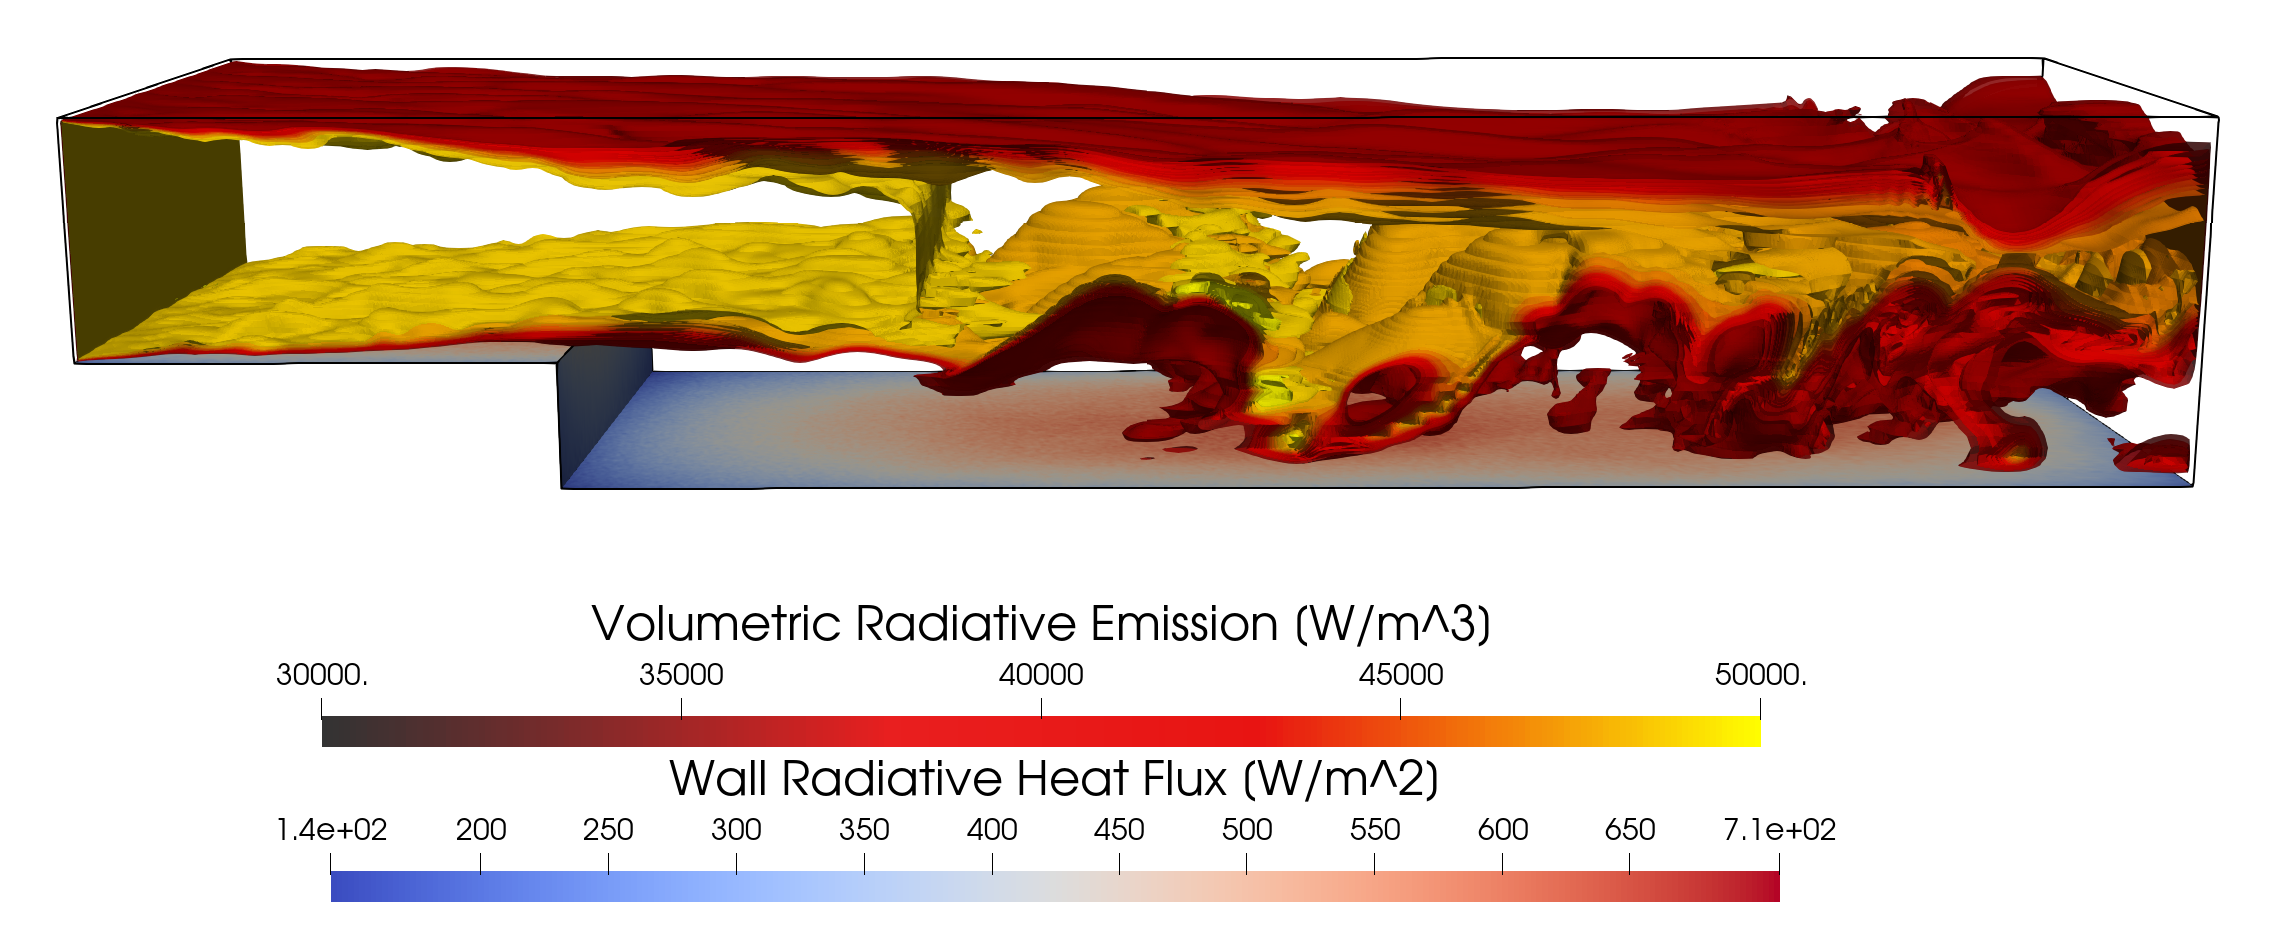
\includegraphics[width=\linewidth]{figures/ch4/BFS_volwallflux3.png}
\caption{Contours of volumetric radiative emission alongside resulting radiative heat flux along the walls.}
\label{fig:PoolFire_diagram}
\end{figure}

\subsection{Results}
Peak radiative emission reaches a value of $15723.3269$ Watts, where $2464.4313$ Watts are re-absorbed into the medium, and $13258.8957$ Watts escape to the walls. This results in roughly 15.6\% of radiative emission being re-absorbed within the flame. Re-absorption fractions reach values up to 0.163\% over all of the timesteps in the simulation.

\section{Additional profiling studies}


- Weak scaling study across many nodes
- Strong scaling within a node, across many nodes
    - Cubic domain, square domain
    - Parallel plates
    
